% ============================================================================
% ALIFE 2026 Late-Breaking Abstract
% The 2026 Conference on Artificial Life (ALIFE 2026),
% Waterloo, Ontario, Canada, 17-21 August 2026.
% Theme: "Living and Life-like Complex Adaptive Systems".
%
% Track: Late-Breaking Abstract. Per the call for papers:
%   - PDF length <= 2 pages for extended/late-breaking abstracts
%     (NOT including citations); consistent US-letter (8.5 x 11 in) pages.
%   - Abstract length <= 250 words.
%   - Reports new ideas / work in progress; reviewed for relevance and quality.
%   - Accepted late-breaking abstracts are presented as posters and are NOT
%     included in the proceedings.
%   - Submission deadline 20 July 2026 (AoE); notification 27 July 2026.
%   - Images <= 300 dpi at 100% scale; embedded fonts; active links; <5 MB.
%
% This file follows the accepted-submission format (alifeconf style) shown in
% the ALIFE 2025 examples supplied by the author.
% If the late-breaking track is double-blind, remove the author block below and
% refer to prior work by the authors in the third person before submitting.
% ============================================================================
\documentclass[letterpaper]{article}

\usepackage{natbib}     %% author-year (apalike), matching the companion paper
\usepackage{alifeconf}  %% The order is important
\usepackage{amsmath,amssymb}
\usepackage{booktabs,graphicx}
\usepackage{url,hyperref,cleveref}  % cleveref must load after amsmath

\graphicspath{{figures/}{../outputs/alife_2026/editable_figures/}{../poster/figures/}}

\DeclareMathOperator*{\argmin}{arg\,min}
\newcommand{\bs}{\mathbf{s}}
\newcommand{\bD}{\mathbf{D}}
\newcommand{\NML}{\operatorname{NML}}
\newcommand{\NLL}{\operatorname{NLL}}

\title{Inside Winnower: Component Semantics of Cellular-Automaton Background
  Decomposition, and the Exact Boundary of Period Inflation}

% Remove/anonymize this block if the late-breaking track is double-blind.
\author{Joshua Herman$^{1}$ \\
\mbox{}\\
$^1$Independent Researcher \\
zitterbewegung@gmail.com}

\begin{document}
\maketitle


\begin{abstract}
A recurring task in artificial life is separating a life-like pattern from the
periodic domain it lives in: a glider is a glider only relative to its
background. \emph{Winnower} is an open-source tool that performs this split on
a cellular-automaton (CA) spacetime, fitting a drifting periodic
\emph{background} by majority vote and returning the \emph{residual mask} of
cells the background cannot explain. We give a component view of the tool in
which each stage of the pipeline --- candidate, orbit classes, majority vote,
background, residual mask, and a complexity-aware score --- is a diagram element
carrying an explicit semantic role. We then address a pressure common to every
fit-based detector, \emph{period inflation}: a longer-period candidate has more
parameters and can never fit worse, so a selector scoring by fit alone drifts
to the largest model. We report a result that pins down exactly when this
pressure exists. For two constant-velocity candidates, five natural conditions
--- velocity-matched divisibility, orbit-partition refinement, model-class
nesting, universal residual improvement, and universal likelihood improvement
--- are all equivalent, and divisibility is \emph{necessary}, not merely
sufficient: whenever it fails, some spacetime makes the longer candidate
strictly worse. The result is proved directly and confirmed by an exhaustive
check over all candidate pairs on a small grid. It is the precise justification
for Winnower's complexity penalty, and it is reproducible in the tool's live
web companion.
\end{abstract}

\begin{figure*}[t]
\centering
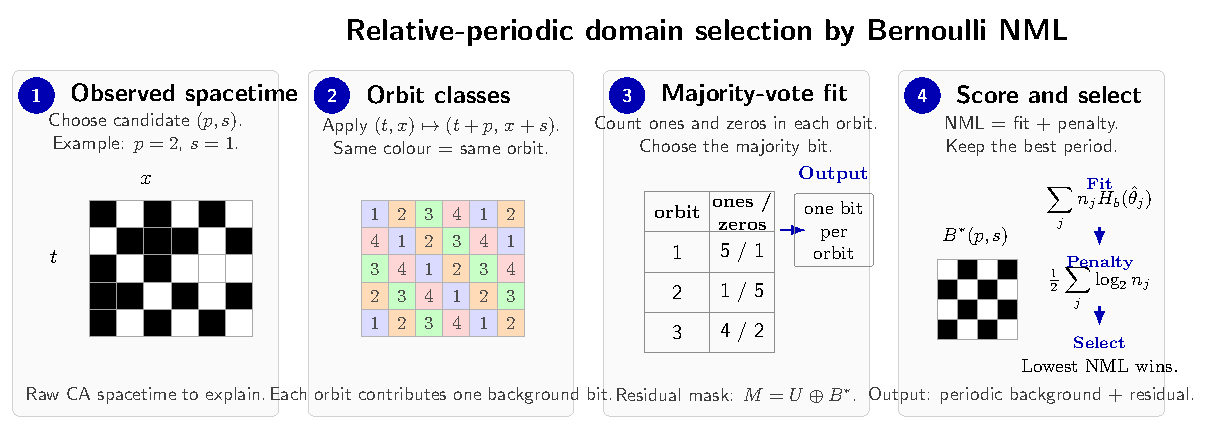
\includegraphics[width=\textwidth]{winnower_nml_figure.pdf}
\caption{How Winnower decomposes a spacetime, in four stages --- each panel a
stage of the pipeline paired with the object it computes and its semantic role.
\textbf{(1)}~A candidate $(p,\bs)$ is chosen and applied to the observed
spacetime $U$. \textbf{(2)}~The induced translation $(t,x)\mapsto(t+p,\,x+\bs)$
groups cells into orbit classes (same colour $=$ same orbit); each class will
contribute one background bit. \textbf{(3)}~A per-class majority vote fixes that
bit, giving the background $B^{*}$ and the residual mask $M=U\oplus B^{*}$ --- the
cells the background cannot explain. \textbf{(4)}~Each candidate is scored by a
Bernoulli NML description length --- fit $\sum_j n_j H_b(\hat\theta_j)$ plus a
complexity penalty $\tfrac12\sum_j\log_2 n_j$ --- and the lowest-scoring period is
selected, returning the periodic background and its residual. Every symbol
($U$, $(p,\bs)$, $B^{*}$, $M$) names an entity referred to in the text, so the
figure doubles as a legend; full derivations are in the companion paper
\citep{winnower2026}.}
\label{fig:pipeline}
\end{figure*}


\section{Introduction}
Cellular automata routinely settle into broad periodic domains threaded with
defects, interfaces, and particle-like activity. For artificial life those
domains are not noise to be discarded but the \emph{reference frame} that makes
coherent structure legible: gliders, spaceships, and their collisions are
defined against the background they traverse
\citep{hanson1992,crutchfield1997}. Extracting that background at scale is a
prerequisite for cataloguing where life-like behaviour appears --- a concern
squarely within the ALIFE 2026 theme of living and life-like complex adaptive
systems.

\emph{Winnower} is a fast global front end for this problem. Given a binary
spacetime $U$ and a grid of \emph{candidates} $(p,\bs)$ --- ``the pattern
repeats every $p$ time steps, drifting sideways by $\bs$'' --- it groups the
cells each candidate forces to be equal (its \emph{orbit classes}), takes a
majority vote in each class to build the best-fitting background $B^{*}$, and
records the residual mask $M = U \oplus B^{*}$. Each candidate costs one linear
pass, so whole-catalogue 1D/2D/3D surveys are practical, and every reported
number re-runs in a browser-based reproduction; the pipeline and full
experimental evaluation are in the companion paper \citep{winnower2026}. This
abstract gives a component view assigning each stage its semantic role
(\cref{fig:pipeline}) and reports an exact characterization of when the
selector's complexity penalty is needed.

\section{The Pipeline, Stage by Stage}
\Cref{fig:pipeline} names each stage of Winnower and the meaning it carries. A
\emph{candidate} $(p,\bs)$ is read as a spacetime translation $\tau$; its
\emph{orbit classes} $\Pi$ are the cells $\tau$ forces to be equal; a per-class
\emph{majority vote} is the Hamming-optimal projection of $U$ onto the model
class $\mathcal{B}(p,\bs)$ of fields constant on classes, yielding the
\emph{background} $B^{*}$ and the \emph{residual mask} $M = U \oplus B^{*}$; and
each candidate is scored by a description length $\NML = \NLL + \text{complexity}$,
the Bernoulli fit plus a normalized-maximum-likelihood penalty for capacity
\citep{shtarkov1987,grunwald2007}, with \emph{selection} returning the
lowest-scoring candidate and its margin. Because every box corresponds to a
named object, the figure doubles as the legend for the rest of this abstract.

\section{An Exact Boundary for the Penalty}
The one design choice that needs justifying is the complexity penalty. Without
it the score reduces to fit, and fit alone is biased. Call $(p_2,\bs_2)$ a
\emph{velocity-matched multiple} of $(p_1,\bs_1)$ when $p_2 = m\,p_1$ and
$\bs_2 = m\,\bs_1 \bmod \bD$: the same drift at a longer period. Such a multiple
splits every orbit class into finer pieces, so its optimal residual count and
its $\NLL$ can only improve, and an unpenalized selector inflates the period
whether or not extra structure is present. We show exactly when this pressure
exists.

Fix a torus with spatial dimensions $\bD$ and temporal length $T$, and two
candidates $c_1,c_2$ acting by translation. Write $\Pi_i$ for the orbit
partition of $c_i$, $\mathcal{B}_i$ for the model class of fields constant on
$\Pi_i$-classes, $d^{*}_U(c_i)$ for the minimum Hamming distance from $U$ to
$\mathcal{B}_i$, and $\NLL_U(c_i)$ for the orbit-class Bernoulli negative
log-likelihood. The following are equivalent:
\emph{(i)}~$c_2$ is a velocity-matched multiple of $c_1$;
\emph{(ii)}~$c_2$'s translation is a power of $c_1$'s;
\emph{(iii)}~$\Pi_2$ refines $\Pi_1$;
\emph{(iv)}~$\mathcal{B}_1 \subseteq \mathcal{B}_2$;
\emph{(v)}~$d^{*}_U(c_2) \le d^{*}_U(c_1)$ for \emph{every} $U$;
\emph{(vi)}~$\NLL_U(c_2) \le \NLL_U(c_1)$ for \emph{every} $U$.

The forward chain (i)$\Rightarrow\cdots\Rightarrow$(vi) is routine
(cyclic-group structure; Jensen's inequality for the concavity of binary
entropy). The content is \emph{necessity}: if divisibility fails, refinement
fails, and a concrete adversarial spacetime --- constant on $\Pi_1$-classes but
mixing two of them inside one $\Pi_2$-class --- makes $c_2$ strictly worse under
both $d^{*}$ and $\NLL$. Closing the loop needs (iii)$\Rightarrow$(ii), that
refinement \emph{forces} a power: on the torus, orbits are cosets of the cyclic
subgroup a translation generates, so refinement at the identity gives subgroup
containment, and a translation is fixed by its value at one point. Divisibility
is thus the exact frontier of the guaranteed-improvement regime --- on one side
longer periods always win, on the other the data can always punish them --- and
hence exactly the set of comparisons the penalty of \cref{fig:pipeline}'s Score
stage must neutralize. We verify the finite-window form of the equivalence by
exhaustively enumerating every candidate pair on a $6\times4$ space--time grid.

\section{Reproducible in the Tool}
The characterization is visible where the tool lives. The same in-browser
reproduction that backs every reported number displays, for any supported rule,
seed, and horizon, the per-period fit ($\NLL$) and penalized ($\NML$) scores
side by side, so a visitor can watch the fit column improve monotonically along
velocity-matched chains --- exactly as predicted --- while the penalized column
resists. At survey scale the effect is stark: on the 105 non-degenerate
Life-like rules at horizon $T{=}100$, selecting by fit alone picks the largest
scanned period for \emph{every} rule, whereas the penalized score concentrates
selections at low period.

\section{Status and Future Work}
This is work in progress. The empirical picture --- planted-ground-truth
recovery at $1.00$ joint accuracy over $642$ runs, zero false positives on
shuffled and random controls --- is established in the companion paper
\citep{winnower2026}. Open threads include extending the analysis from pairwise
comparisons to the full candidate lattice the scanner searches, and relaxing the
nondegeneracy hypothesis ($p_2 \le T-1$) in the finite-window form. The tool,
code, tests, and in-browser reproduction are public.

\footnotesize
\setlength{\bibsep}{2pt plus 0.3ex}
\bibliographystyle{apalike}
\begin{thebibliography}{9}

\bibitem[Crutchfield and Hanson, 1997]{crutchfield1997}
Crutchfield, J.~P. and Hanson, J.~E. (1997).
Computational mechanics of cellular automata: An example.
\emph{Physica D}, 103:169--189.

\bibitem[Gr{\"u}nwald, 2007]{grunwald2007}
Gr{\"u}nwald, P. (2007).
\emph{The Minimum Description Length Principle}. MIT Press.

\bibitem[Hanson and Crutchfield, 1992]{hanson1992}
Hanson, J.~E. and Crutchfield, J.~P. (1992).
The attractor-basin portrait of a cellular automaton.
\emph{Journal of Statistical Physics}, 66:1415--1462.

\bibitem[Herman, 2026]{winnower2026}
Herman, J. (2026).
Winnower: A fast tool for splitting cellular automaton spacetimes into a
periodic background and a residual mask.
Companion manuscript; source, data, and in-browser reproduction at
\url{https://github.com/zitterbewegung/Winnower}.

\bibitem[Shtarkov, 1987]{shtarkov1987}
Shtarkov, Y. (1987).
Universal sequential coding of single messages.
\emph{Problems of Information Transmission}, 23:3--17.

\end{thebibliography}

\end{document}
